\chapter{Prototyping and Testing}

\section{Simulation Results}

As previously discussed, the developed MATLAB model featured a winter and summer scenario to estimate the theoretical performance of the DX-SAHP system. The results of the simulation indicate that the system would be capable of provisioning 1.1 KWh of power with an average $COP$ of 2.4 for the winter scenario. During the summer months, when irradiance levels are higher, and ambient temperatures are warmer, the system would be able to generate 2 KWh of power with an average $COP$ of 3.0, virtually satisfying the entirety of the hot water heat load demand ($\sim2KW$). The collector efficiency was also determined to range between 51\% to 74\%, which is comparable to the efficiency of locally manufactured flat plate solar thermal collectors. The figure below depicts the performance of the DX-SAHP system during a harsh winter day with low irradiance levels, confirming the feasibility of the system for cold climates. 

\medskip
\begin{figure}[H]
    \centering
    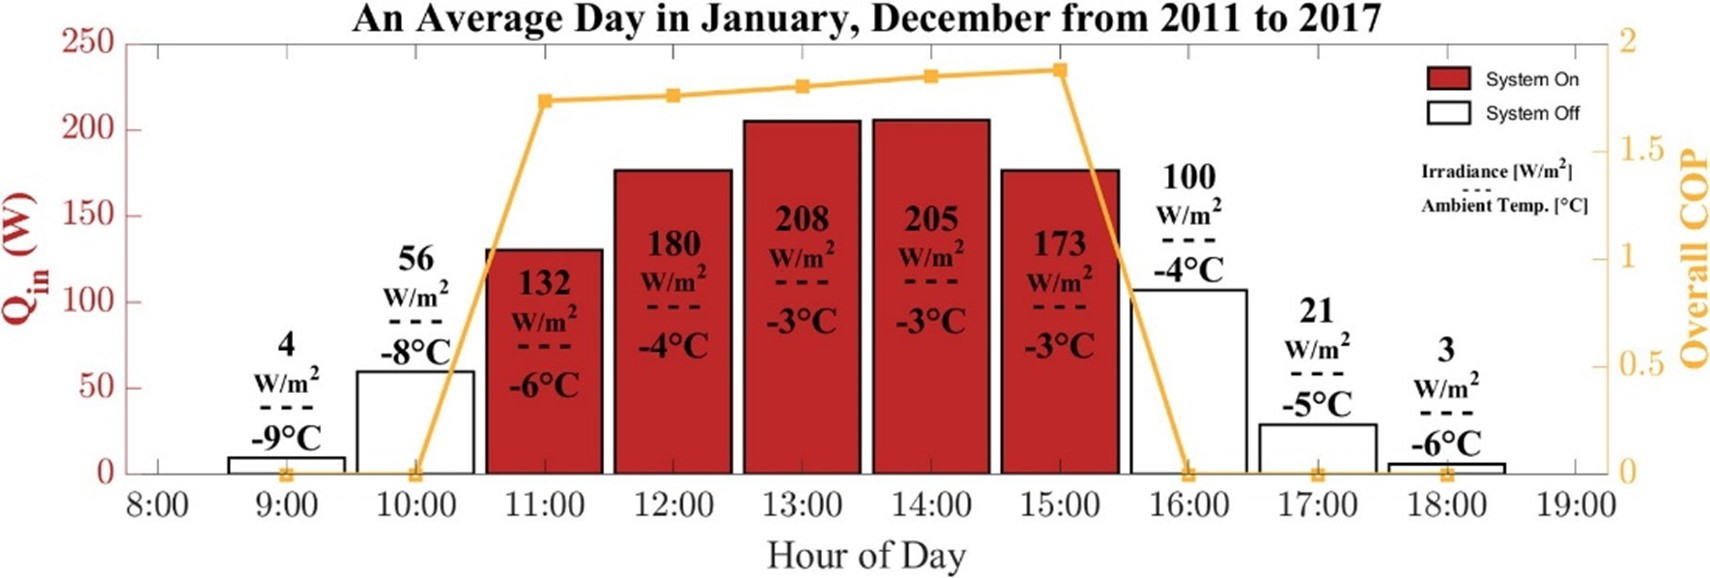
\includegraphics[width=\textwidth]{images/simulation.jpg}
    \caption{Simulation Results for an Average Winter Day}
\end{figure}

\section{Developed Prototype}
\subsection{Refrigeration Assembly}
\subsubsection{Aluminum Absorber Plate to Copper Manifold Bonding}

The bonding of the copper tubing to the aluminum plate was necessary as to minimize any air gaps present that would affect the thermal performance of the system. The method of bonding was evaluated based on the following options:

\medskip
\begin{enumerate}[itemsep=3mm, parsep=-1mm, label=\roman*.]
    \item Brazing or Soldering.
    \item Thermally Conductive Epoxy Adhesive.
    \item Copper Strapping with Threaded Steel Galvanized Screws.
\end{enumerate}

\medskip
Due to the dissimilar thermal properties of the two metals, brazing copper to aluminum is not a suitable option. The appropriate brazing technology and flux must be used for this process to be applicable. The issues with brazing copper to aluminum is mainly due to aluminum having a much lower melting point than copper. The melting points of aluminum and copper are respectively, approximately $650$ \textdegree C and over $1000$ \textdegree C. The flame is typically directed on the copper and as heat transfers from the copper to the aluminum, the copper tends to melt quicker while copper is still absorbing the heat. This process accelerates the destruction of the aluminum components \cite{brazingALCU} and results in an insufficient bond.

\medskip
For additional expertise, the team contacted several companies including those who deal with specialized welding. The option of brazing or soldering the two dissimilar metals was advised against.

\medskip
The second option of thermally conductive epoxy adhesives was then considered. Mainly, epoxy adhesives are used for leaks or refrigeration repairs and thorough research was applied into determining the type of product to use for this application. The investigation into selecting a thermally conductive epoxy adhesive was based on the highest thermal conductivity to later achieve better thermal performance of the system, substrate compatibility, room temperature curing, and having a strong bond. The viscosity of the product to be considered was to be of paste form.

\medskip
A thermally conductive silver epoxy  adhesive was evaluated. This two-part product consisted of a one-hour work time, room temperature curing for 24 hours, and was within a temperature range suitable for the system. This product was an excellent choice for aluminum and copper as well as having a thermal conductivity value of $500 W/m^2K$. This product did not work for bonding the copper tubing to the aluminum plate.

\medskip
The team then evaluated the option of securing the copper tubing to the aluminum plate by use of copper strap. The copper strapping was snipped into tiny, flexible brackets which were then drilled into the aluminum plate by use of threaded steel galvanized screws. The screws extending outwards on the opposite end of the plate were then grind and polished.

\medskip
A thermal mastic heat transfer compound was evaluated as the final selection into minimizing the air gaps that were still present due to the copper tubing not being flush with the aluminum plate. The thermal conductivity of this product was not as high as the silver epoxy, however, was quite higher than air and this is mainly what was required. This paste compound did not require curing, does not harden, and does not lose adhesion. This product was applied throughout the entire length of tubing to minimize the air gaps.

\medskip
The following table shows the specifications of the two heat transfer compounds.

\medskip
\begin{table}[H]
\centering
\caption{Specifications - Heat Transfer Compounds}
\rowcolors{2}{gray!20}{white}
\begin{tabular}{|P{60mm}|P{45mm}|P{45mm}|}
    \hline
    \rowcolor{orangeRed}
     & Silver Epoxy Adhesive & Thermal Mastic Compound \\
    \hline
    \textbf{Cure Schedule} & 24h at Room Temperature & N/A \\
    \textbf{Operating Temperature $\SI{}{\celsius}$} & -50 to +170 & -45 to +100 \\
    \textbf{Viscosity} & Paste & Paste \\
    \textbf{Thermal Conductivity $[W/m^2 K]$} & $\sim500$+ & $\sim37$ \\
    \hline
\end{tabular}
\end{table}

\medskip
The following figure shows the final bonding of the copper tubing to the aluminum plate.

\medskip
\begin{figure}[H]
    \centering
    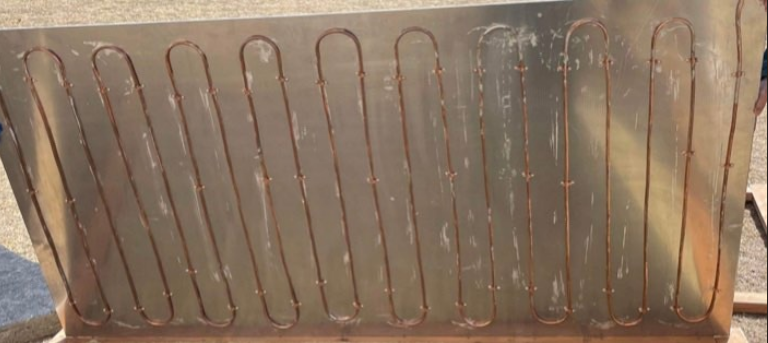
\includegraphics[width=10cm]{images/manifold.png}
    \caption{Bonding - Copper Tubing to Aluminum Plate}
\end{figure}


\subsubsection{Casing}

The casing of the collector frame was made with 2x4 lumber and a plywood pine board. The casing was built following the engineering drawing created for assembly - where the finalized rectangular dimensions were: $2.2m \times 1.3m$. With these dimensions, a SOLIDWORKS strain analysis was conducted to determine the maximum deflection of the 5052 H2 aluminum plate sitting on top of the frame. Knowing the weight of the aluminum plate (29.48kg) and the weight of the copper manifold (1.61kg), a point load was applied at the center to determine the maximum deflection of the plate and in turn determine if the dimensions of the casing were still suitable. Although at first glance, the casing is simply a rectangular enclosure, creating the casing was much more difficult than was expected. First the wood was treated with a stain and sealer to prevent rotting in the outside conditions. As the casing was created in a garage without access to proper shop tools such as a planar, the process of creating the casing was much more difficult due to the warped raw lumber. This was counteracted with the use of multiple clamps and PL Premium wood glue.

\begin{figure}[ht]
    \centering
    \subfloat[\centering Collector Engineering Drawing] {{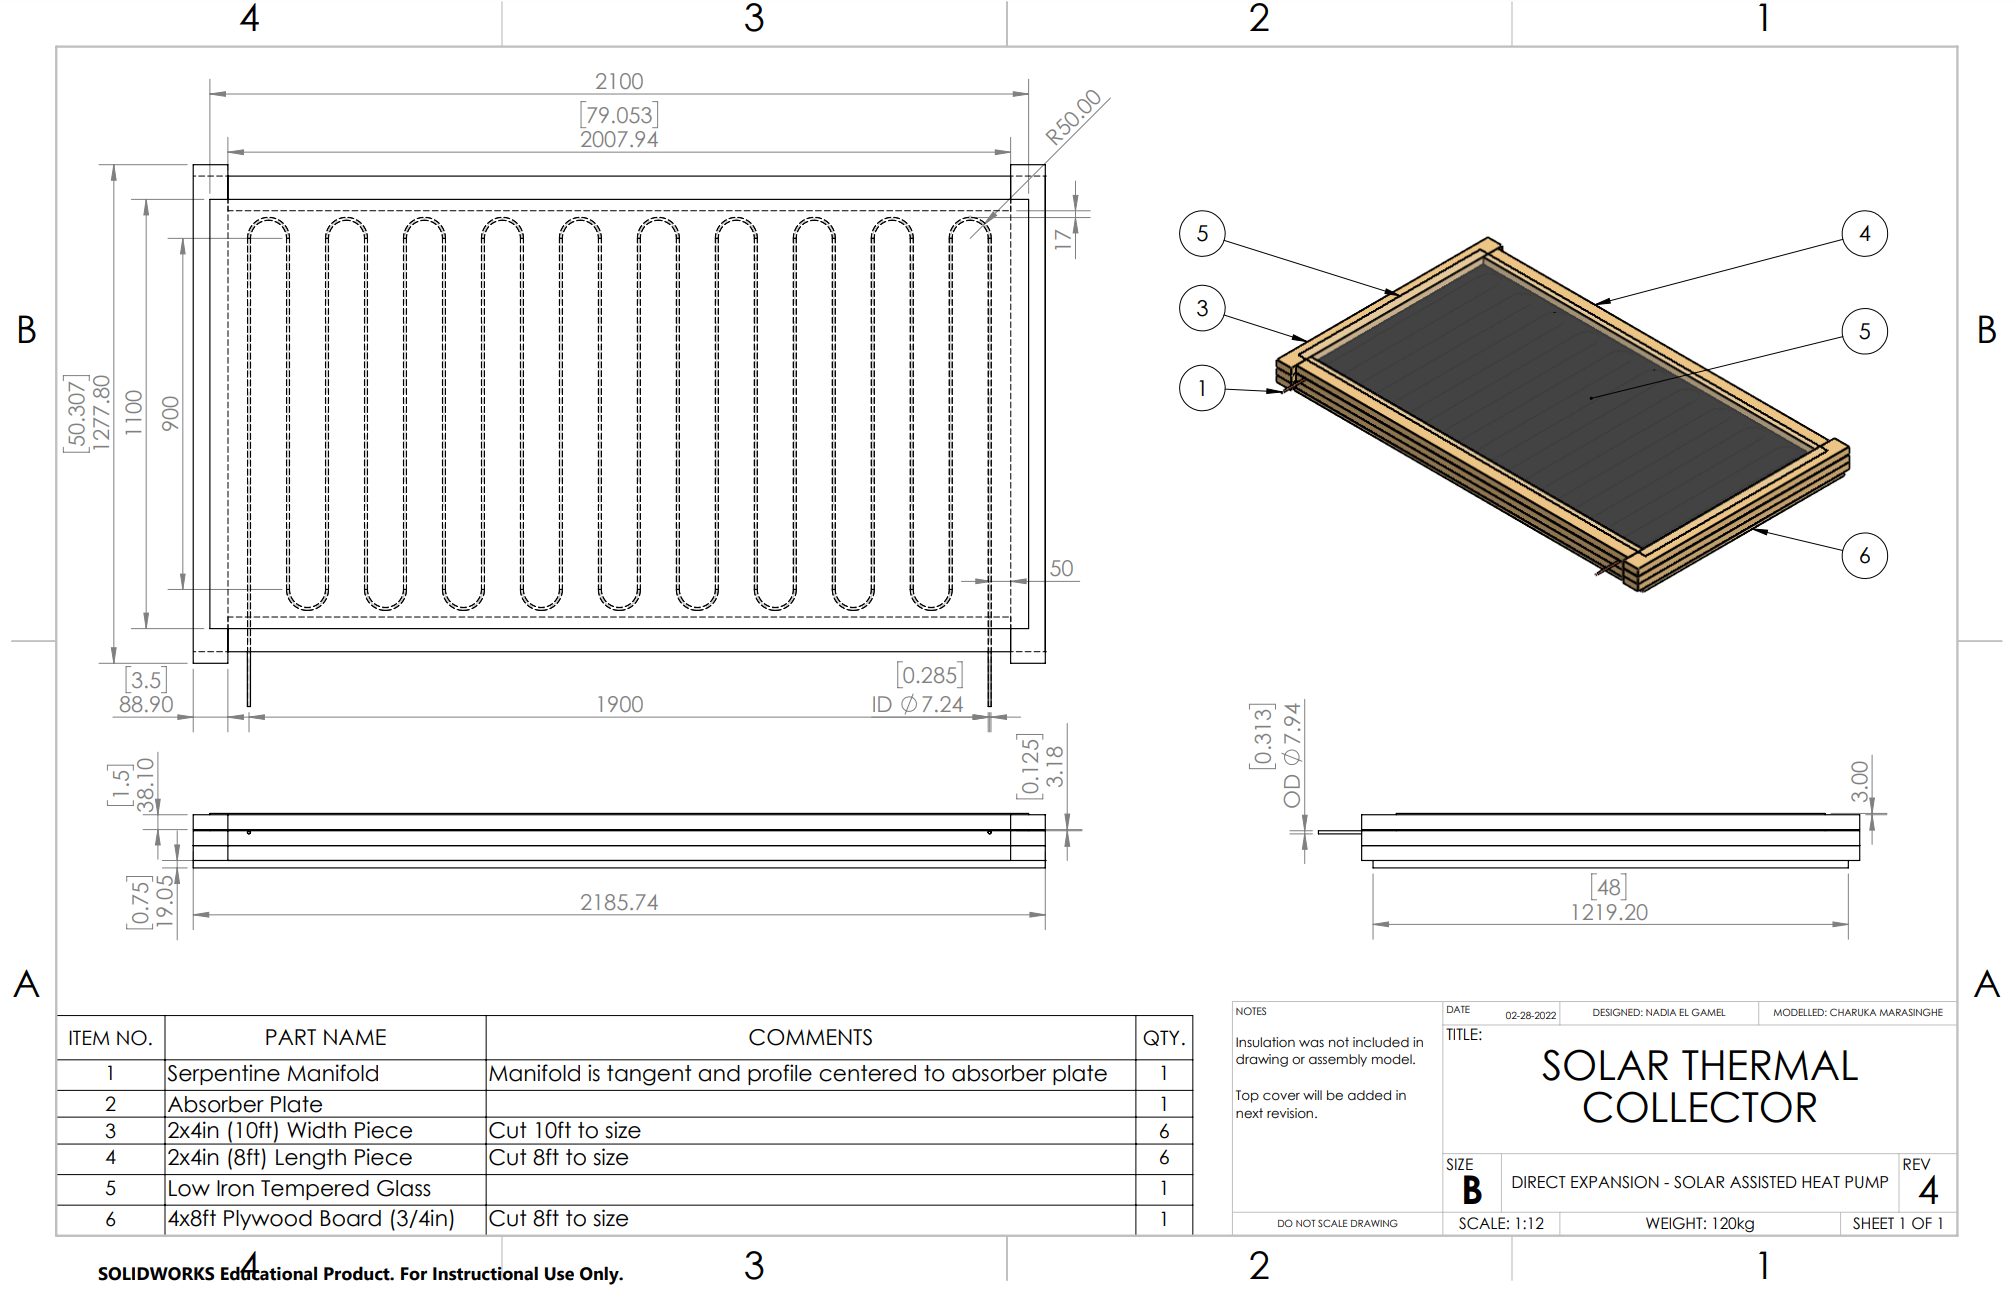
\includegraphics[height=6.5cm]{images/collecter_drawing.PNG}}}
    \qquad
    \subfloat[\centering Collector Wood Casing] {{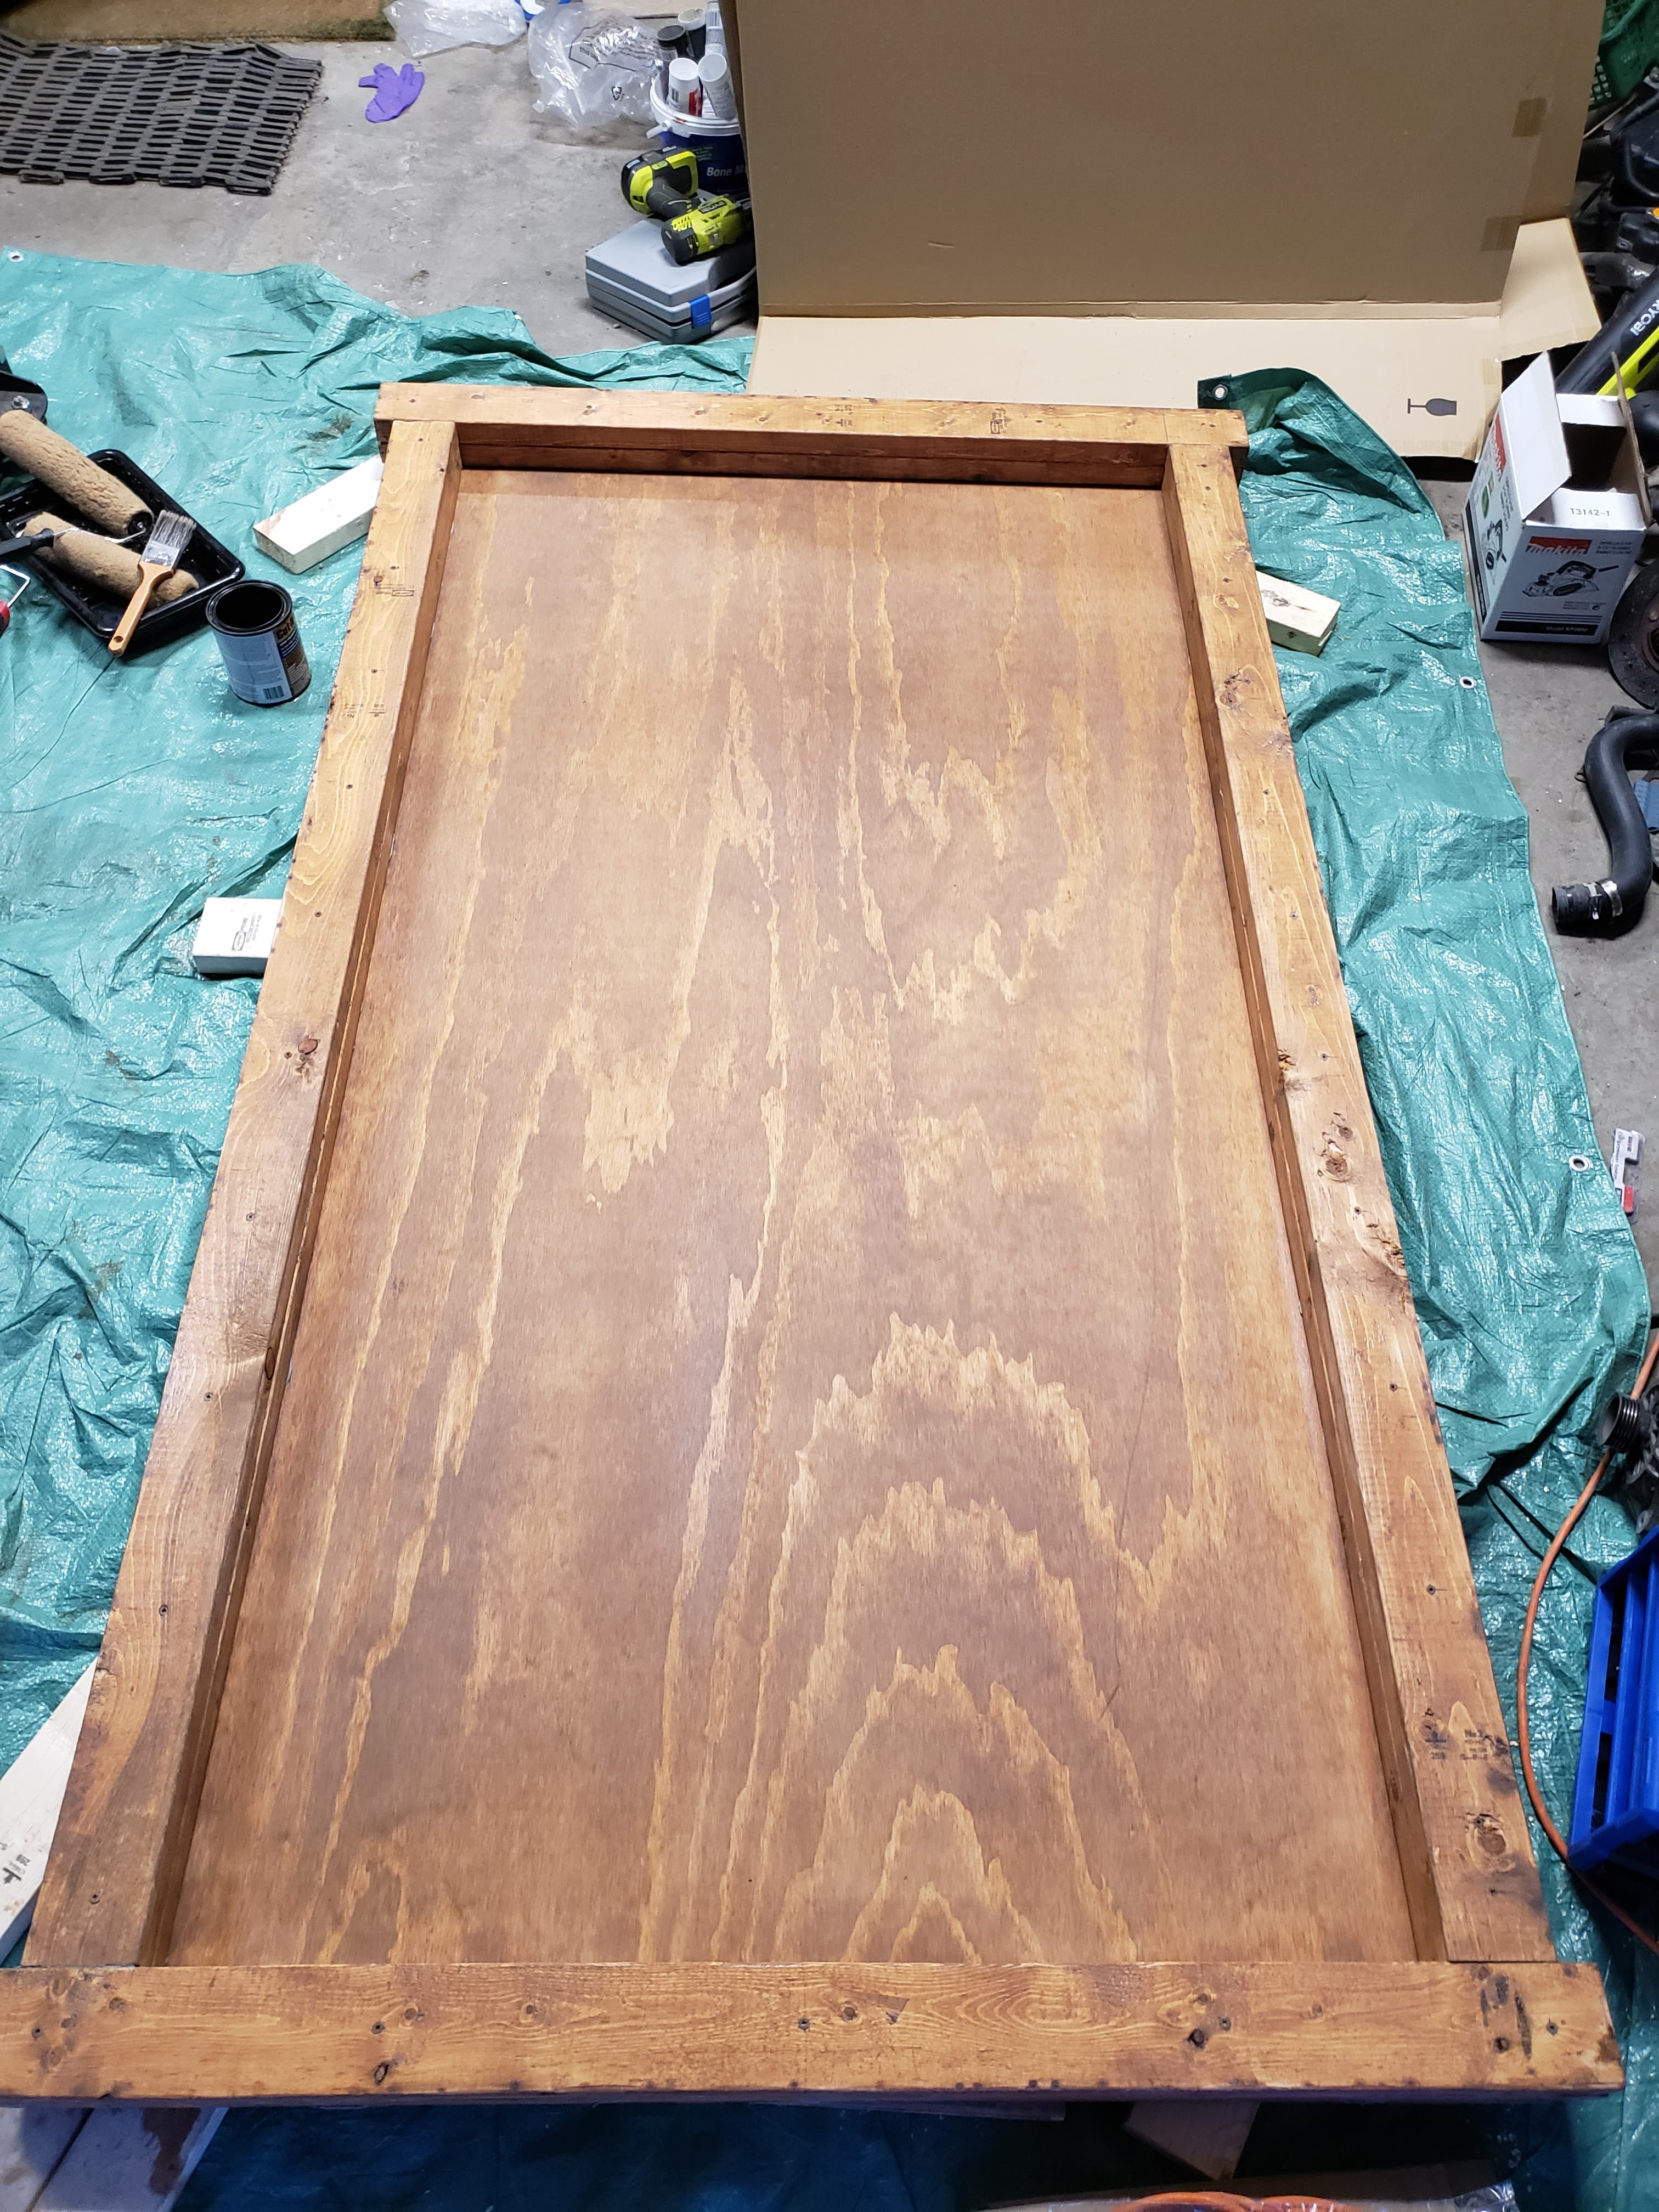
\includegraphics[height=6.5cm]{images/collector_casing.jpg}}}
    \caption{Solar Thermal Collector Design and Fabrication}
\end{figure}

\subsubsection{Frame}

With the Solar Thermal Collector fully assembled, the final weight was determined by simply adding up the combined weights of all components in the collector:

\medskip
\begin{table}[H]
\centering
\caption{Solar Thermal Collector Weights}
\rowcolors{2}{gray!20}{white}
\begin{tabular}{|P{75mm}|P{75mm}|}
    \hline
    \rowcolor{orangeRed}
    Component & Weight $(kg)$ \\
    \hline
    Wood Casing & 61.49 \\
    Absorber Plate Manifold & 31.09  \\
    Glass Glazing & 17.53 \\
    \textbf{Total Combined Weight} & \textbf{110.11kg} \\
    \hline
\end{tabular}
\end{table}

\medskip
Knowing the weight and dimensions of the solar thermal collector, the frame could now be designed. The team first sent these requirements to an external vendor to help create the frame, but was quoted for \$5600. Due to the high price tag of the frame, it was decided that with the help of the Schulich School of Engineering's Makerspace Machine Shop, a frame would be designed and welded in house.

\medskip
The primary failure mode in the frame to be concerned on is column buckling due to the heavy load of the solar collector. To determine the sizing of the steel tubes, the Euler Buckling Equation was utilized with an effective length of 0.25 as a fixed/free end system:
\begin{align}
    F_cr = \ddfrac{\pi ^2 EA}{(\ddfrac{k_{eff}L}{r})^2}
\end{align}
\medskip

Applying the weights on the steel frame distributed evenly across the 4 columns from the preliminary design of the frame as the critical loads, the critical cross sectional area of the tubing was able to be determined. To allow for ease of assembly, and to be conservative in the calculations, it was determined that 1.5" tubing would be more than sufficient in preventing the frame from failing.

\medskip
Knowing the sizing of the steel tubing required, the frame was modelled with 3 key factors in mind:

\medskip
\begin{enumerate}[itemsep=3mm, parsep=-1mm, label=\roman*.]
    \item Easy to disassemble.
    \item Easy to move.
    \item Able to change tilt angle between 45\textdegree and 51\textdegree.
\end{enumerate}

With these criteria, the following frame was designed:

\begin{figure}[H]
    \centering
    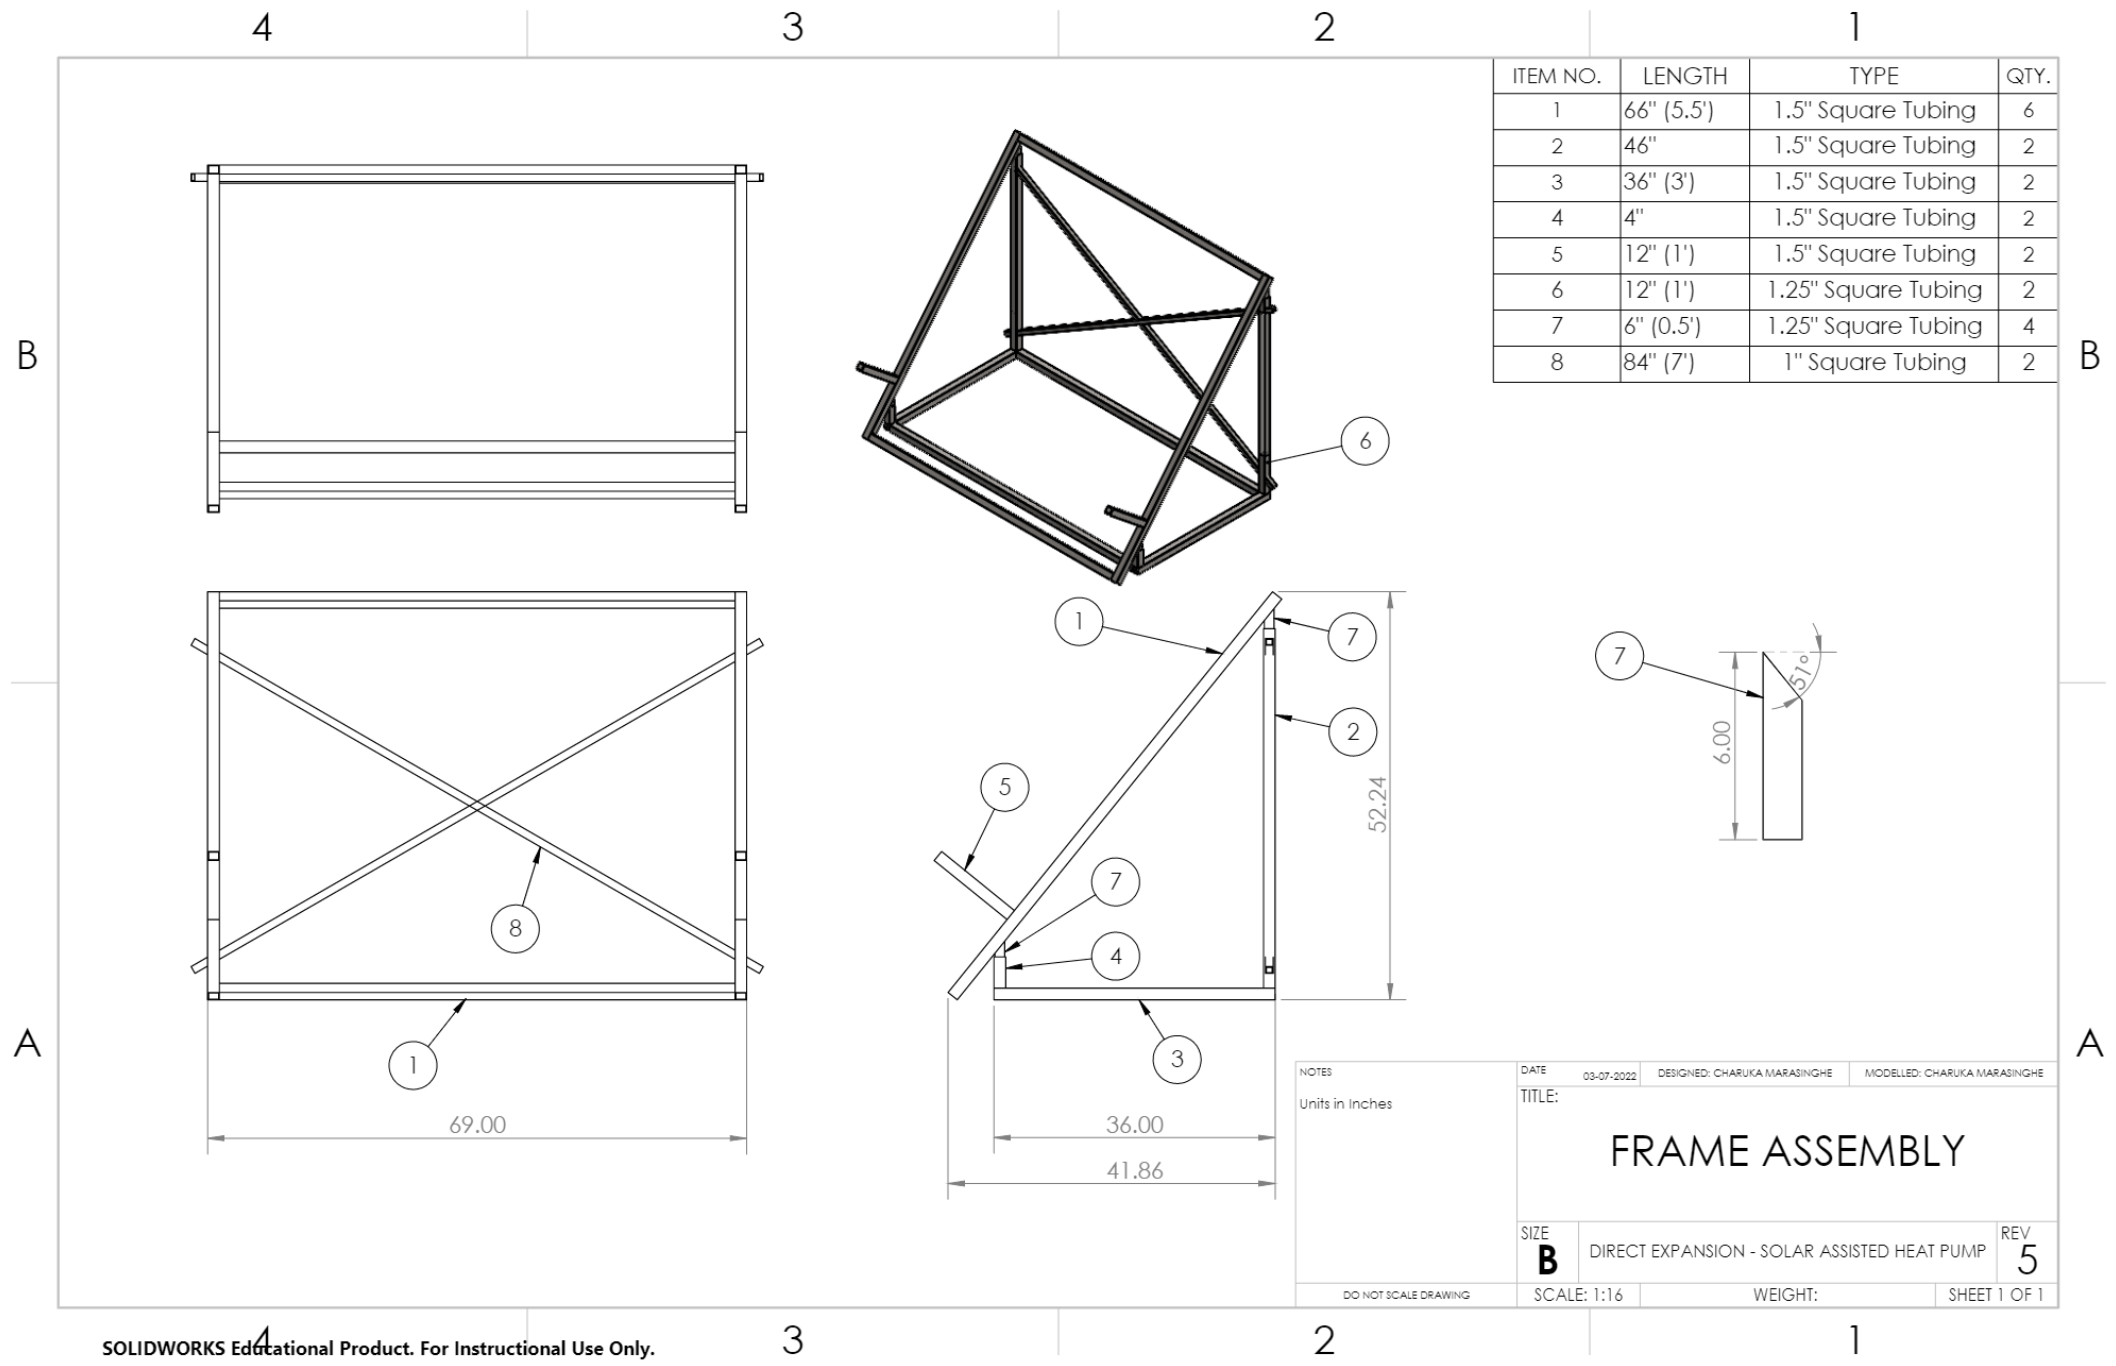
\includegraphics[width=\textwidth]{images/frame_drawing.PNG}
    \caption{Assembly Frame Engineering Drawing}
\end{figure}

\medskip
The assembly was designed in 3 frames with telescoping joints to easily take apart and put back together. Using caster wheels rated for over 1300lbs attached to a steel plate, the system was easily movable. However, the final challenge came in designing the pivot joints to allow for varying tilt angles. Because the solar collector had a piping manifold with refrigerant running through it and was brazed to the other system components, tilting the collector with the frame, would mean the entire system would tilt as well. This is not possible as the other major components of the system were fixed onto the steel base plate.

\medskip
Using the engineering drawings, and cutting the tubing accordingly, the frame was MIG (metal inert gas) welded together. To prevent rusting due to the outside conditions, the frame was also spray painted. With the frame completed, the solar collector was then lifted and placed onto the support members of the frame as seen below.

\begin{figure}[H]
    \centering
    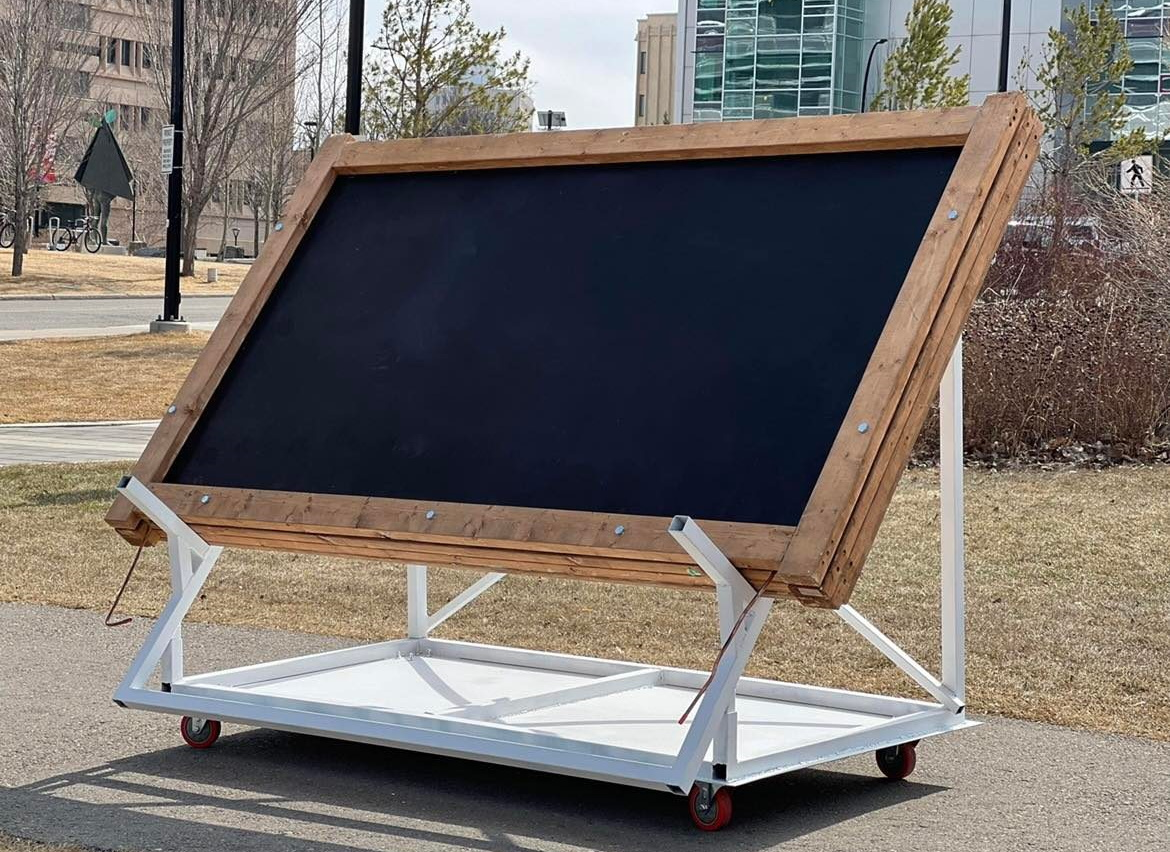
\includegraphics[width=12.5cm]{images/frame_assembly.jpg}
    \caption{Assembly Frame}
\end{figure}


\subsubsection{Heat Pump Assembly}

External sponsorship was provided by Emerson, supplying the team with many refrigeration components and assistance such as:

\medskip
\begin{enumerate}[itemsep=3mm, parsep=-1mm, label=\roman*.]
    \item Fixed Speed Scroll Compressor.
    \item Pulse Width Modulation Electronic Expansion Valve.
    \item Superheat Controller.
    \item Labour required for piping and the assembly of the refrigeration cycle,.
    \item Leak and pressure testing.
    \item Evacuation/Charging and commissioning of the refrigerant, R-134a.
\end{enumerate}

\medskip
The following figure shows the heat pump assembly for the refrigeration cycle of the DX-SAHP. In the figures below, the heat pump cycle is comprised of four major components – the solar thermal collector, fixed speed scroll compressor, coaxial coil, and the electronic expansion valve. The assembly of the refrigeration cycle consists of the piping that is connected from the outlet of the solar thermal collector to the compressor. The piping to and from the compressor is connected to valves allowing for the compressor to be disassembled in case of any maintenance issues. The piping then leads to the coaxial coil in which the refrigerant exchanges heat with the water. Further, the piping is connected to auxiliary components such as, the receiver, filter drier, and sight glass. Lastly, the piping connects to the electronic expansion valve for the cooled refrigerant to become depressurized. This piping is then connected to the outlet of the solar collector via the copper serpentine manifold attached beneath the aluminum absorber plate. The piping was attached by auxiliary piping connections (i.e., couplings) and fittings as well as brazing.

\medskip
\begin{figure}[H]
    \centering
    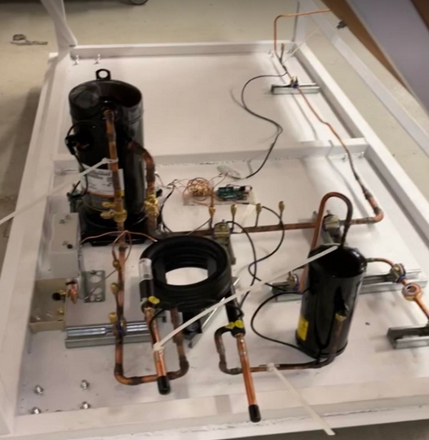
\includegraphics[width=6cm]{images/heat_pump_assembly.png}
    \caption{Heat Pump Assembly for the DX-SAHP}
\end{figure}

Figure 4.7 shows the final heat pump assembly of the DX-SAHP connected to the piping in the solar thermal collector.

\medskip
\begin{figure}[H]
    \centering
    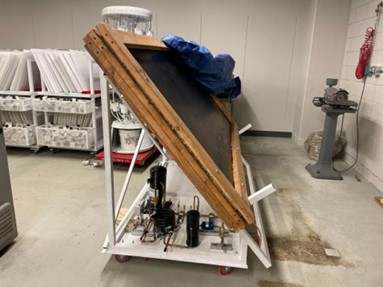
\includegraphics[width=10cm]{images/assembly.jpg}
    \caption{Full Assembly for the DX-SAHP}
\end{figure}

\subsection{Water Circulation Assembly}

Due to uncertainties with the refrigerant side piping, the layout of the water side was to be determined after. Estimates on the pipe lengths were made to do preliminary calculations. Once the refrigeration side is finalized, measurements will be taken to determined exact pipe lengths and components (i.e., elbows and couplings) required. The piping assembly will be completed using Sharkbite connections which are easy to assemble as they are push-to-fit. Since PEX piping will expand and contract with changes in temperature, care will be taken during installation to ensure there is adequate room to allow for this change in length (1” to 2.5” every 100’).

Once the water side piping is complete, testing can begin.


\subsection{Data Acquisition System}
\subsubsection{Design Validation Goals}

To verify the design and determine the system performance, a data acquisition system was developed. The COP of the DX-SAHP can be defined as,

\begin{align}
    COP = \ddfrac{Q_{out}}{W_{cycle}} = \ddfrac{\dot m (h_2 - h_3)}{\dot m (h_2 - h_1)} = \ddfrac{(h_2 - h_3)}{(h_2 - h_1)}
\end{align}

\medskip
As evidenced by Equation 4.1, the $COP$ of the system can be determined knowing the specific enthalpy of the refrigerant at certain points. Specific enthalpy at any location can be found through use of temperature and pressure measurements and the refrigeration table of R-134A [18]. As so, temperature sensors at 3 locations (1, 2, 3) and pressure sensors at 2 locations (1, 2) on Figure 4.1 below will be used to determine $COP$. The pressure sensor at 3 can be neglected under the isobaric condensation assumption. However, a temperature sensor at 3 is still necessary as it is pertinent to know and minimize the degree of sub-cooling at the inlet of the electronic expansion valve. Additionally, pressure transducers are approximately at least 20 times more expensive than a thermistor at any given location, so the isobaric assumption was also used for economic reasons.

\medskip
In the above $COP$ equation, it was assumed that all the power input into the compressor is going into superheating the refrigerant. This in fact is not valid, as the compressor itself will hold an efficiency factor. This efficiency factor dictates how much power the compressor puts into the refrigerant, from the total power it uses. To evaluate this efficiency factor, the following equation will also be used to determine $COP$,
\begin{align}
    COP = \ddfrac{Q_{out}}{W_{cycle}} = \ddfrac{\dot m_{water}C_p(T_{water, out}-T_{water, in})}{W_{cycle}}
\end{align}

\medskip
To determine COP using Equation 4.2, the mass flow rate of the refrigerant and the power consumption of the compressor must additionally be known. The mass flow rate of the water can be found from the head that the water pump drives at, from its data sheet. To measure the temperature of the water, two additional thermistors can be placed at the coaxial coil’s inlet and outlet. Additionally, a power meter can be connected to the compressor to determine power usage. This equation will lead to a very conservative value of $COP$, as the heat rejection of the heat pump is calculated from the heat gain of the water. Nevertheless, as it was not feasible for the team to determine the refrigerant’s mass flow rate, this strategy had to be used.

\medskip
To verify the design, a $COP > 2.3$ and a water outlet temperature of 55ºC needs to be constantly achieved, as per design requirements. The afore-described strategy will assist in quantifying design verification.

\subsubsection{Sensor Selection and Placement}
\medskip
Figure 4.1 below provides a visual guide of sensor placements in the system.

\medskip
\begin{figure}[H]
    \centering
    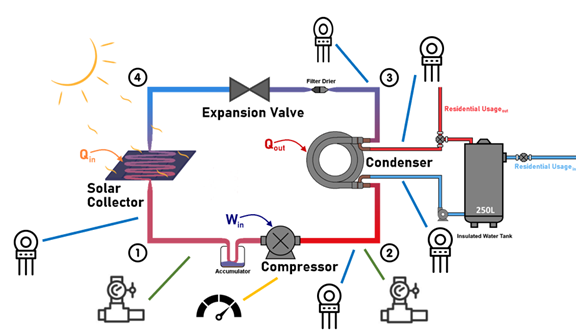
\includegraphics[width=12.5cm]{images/sensor_locations.png}
    \caption{Sensor Locations}
\end{figure}

\medskip
To get the data outputs from the sensors, several data acquisition configurations were explored. Ultimately, an Arduino Uno was decided upon as the data acquisition device as it was the most economical option. Arduino Uno’s have only six analogs to digital converter (ADC) pins, whereas at least eight ADC pins would have been needed if all selected sensors gave analog outputs. To bypass this issue, digital thermistor sensors that could be connected to digital pins on the Arduino were chosen instead. Arduino Uno ADC pins have a maximum bit size of 12, which can affect resolution of the measurement picked up. For all the analog sensors chosen, this resulted in the smallest magnitude that could be measured being 1-2\% of the expected value. This resolution was decided to be sufficient for the needs of the data acquisition system. Table 4.1 shows a full list of sensors used. Note that the location numbering refers to schematic in Figure 4.1.

\medskip
\begin{table}[H]
\centering
\caption{List of Sensors to be used in Data Acquisition System}
\rowcolors{2}{gray!20}{white}
\begin{tabular}{|P{26mm}|P{26mm}|P{15mm}|P{27mm}|P{23mm}|P{20mm}|}
    \hline
    \rowcolor{orangeRed}
    Sensor Type & Location(s) & Accuracy & Operating Range & Power Supply & Output Type \\
    \hline
    Thermistor \textbf{DS18B20} & 1, 2, 3, Water Inlet, Water Outlet        & $\pm \SI{0.5}{\celsius}$ & $\SI{-55}{\celsius}$ to $\SI{125}{\celsius}$ & Arduino  & Digital \\
    Pressure Transducer \textbf{P/N 800-2100}   & 1                            & 0.25\%                   & $0psi$ to $100psi$ & $9V$ to $30V$ DC at $<10mA$ & Analog $0V$ to $5V$ DC \\
    Pressure Transducer \textbf{P/N 800-2500}   & 3                            & 0.25\%                   & $0psi$ to $500psi$ & $9V$ to $30V$ DC at $<10mA$ & Analog $0V$ to $5V$ DC \\
    Power Meter \textbf{Power Meter Buster} \cite{power_meter}           & Compressor Electrical Outlet & 3\%                      & 0KWH to 9999KWH & Compressor Power Supply  & Screen Display \\
    \hline
\end{tabular}
\end{table}

\medskip
An external power supply will have to be used for the pressure transducers. The two pressure transducers were supplied by the team’s industry sponsor, Emerson. For more information on the different sensors that were explored, please see the Sensor Selection excel file in the Design Binder.

\subsubsection{Prototype DAQ Setup}
Figure 4.2 shows the DAQ implemented in the prototype. This DAQ records sensor readings every 30 minutes and stores them in a micro-SD card. During testing, someone would have to come at 30-minute intervals and also manually record the power usage of the compressor from the power meter’s digital display. Once the testing period is over, the data can be compiled and analyzed to determine the $COP$ of the prototype in 30-minute increments. This is useful as the ambient temperature’s effect on the $COP$ can then be observed.

\medskip
\begin{figure}[H]
    \centering
    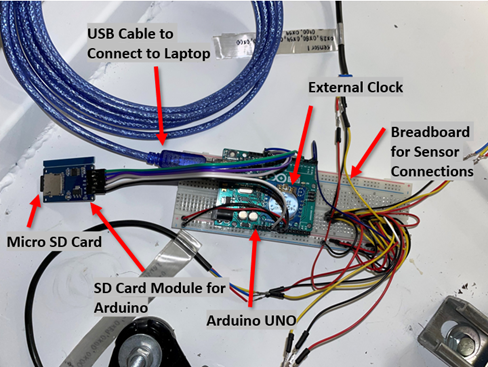
\includegraphics[width=9cm]{images/daq_prototype.png}
    \caption{DAQ Setup in Prototype}
\end{figure}

There were several modules that had to be added to the Arduino Uno. Firstly, a RTC module was connected, to keep more accurate time keeping. As the Arduino Uno is coded to record data every 30 minutes, having an accurate time keeping module was necessary. Secondly, as the Arduino does not have much storage, a SD card module and a micro-SD card were added so that the recorded sensor readings could be stored in the card. This card can then be connected to any computer and the recorded data could be read onto an Excel file. Wiring of the SD card module and code for the SD card writing was created with help from [2]. The Arduino Uno will also be connected to a 5 Vdc battery bowered power supply, so it can be on, even when not connected to a laptop.

\medskip
For more information on how to use the Arduino Uno for data acquisition, please see the User Manual in the design binder. 

\medskip
Please note that currently the Arduino code that has been developed has only been tested for use with the temperature sensors. Once the pressure sensors arrive and are hooked up to the Arduino Uno, they should be individually tested with brand new code, and once that testing is successful, that code can be appended to the main code. Due to supply chain logistics impacted by the COVID-19 pandemic, there has been trouble sourcing some electronic equipment, which is why the superheat controller, and the pressure transducers were not able to arrive on time.

\subsubsection{Temperature Sensor Wiring and Placement}
The code to read the outputs for the temperature sensors was created with help from an online library \cite{temp_library} and other resources that are available for the DS18B20 digital thermistors \cite{temp}. Multiple sensors were able to be hooked up to the same Arduino Uno digital input port, using the following wiring diagram from \cite{mult_temp}:

\medskip
\begin{figure}[H]
    \centering
    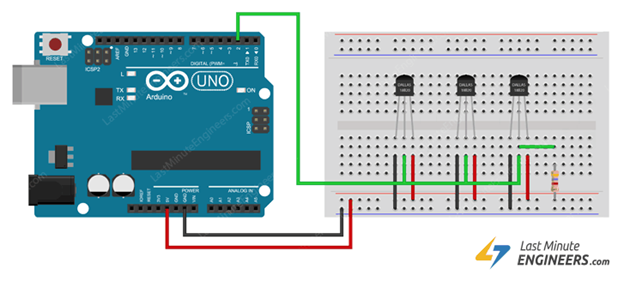
\includegraphics[width=12cm]{images/arduino_thermistors.png}
    \caption{Hooking up Multiple DS18B20 Thermistors \cite{mult_temp}}
\end{figure}

\medskip
Figure 4.4 below shows how the thermistor probes were setup in the actual prototype. The probes were placed as close as possible to the copper piping in the longitudinal direction, and then were strapped in using zip ties. This method was one of the ones suggested from \cite{temp_place}, who work extensively with these digital thermistors in HVAC applications. It is of note that insulating the probes or creating a copper envelope for them to stick into, would lead to obtaining more accurate values, and this is something that can be implemented in future iterations.

\medskip
\begin{figure}[H]
    \centering
    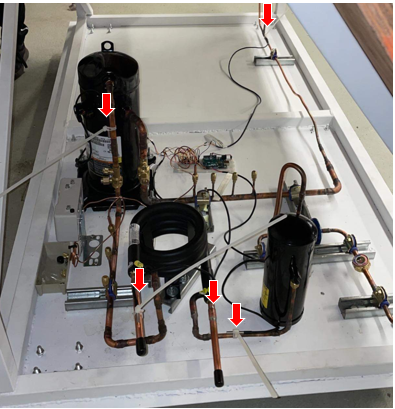
\includegraphics[width=8cm]{images/prototype_daq_locations.png}
    \caption{Prototype Thermistor Locations (marked with arrow)}
\end{figure}

\subsection{Bill of Materials}

Please see the Bill of Materials attached to the appendix.